%!TeX root=../tese.tex
%("dica" para o editor de texto: este arquivo é parte de um documento maior)
% para saber mais: https://tex.stackexchange.com/q/78101/183146

% Apague as duas linhas abaixo (elas servem apenas para gerar um
% aviso no arquivo PDF quando não há nenhum dado a imprimir) e
% insira aqui o conteúdo dos apêndices do seu trabalho (ou deixe
% este arquivo vazio)

% Os apêndices podem ser inseridos diretamente aqui ou "puxados" de outros
% arquivos.
% Em alguns (raros) casos, pode ser interessante usar \include ao
% invés de \input: https://tex.stackexchange.com/a/32058/183146

% %!TeX root=../tese.tex
%("dica" para o editor de texto: este arquivo é parte de um documento maior)
% para saber mais: https://tex.stackexchange.com/q/78101/183146

\chapter{Código-Fonte e Pseudocódigo}
\label{ap:pseudocode}

Com a \textit{package} \textsf{listings}, programas podem ser inseridos
diretamente no arquivo, como feito no caso do Programa 4.1 %~\ref{prog:java},
ou importados de um arquivo externo com o comando
\textsf{\textbackslash{}lstinputlisting}, como no caso
do Programa~\ref{prog:mdcinput}.

% O exemplo foi copiado da documentação de algorithmicx
\begin{program}
  \lstinputlisting[
    language=pseudocode,
    style=pseudocode,
    style=wider,
    functions={},
    specialidentifiers={},
  ]
  {conteudo-exemplo/euclid.psc}

  \caption{Máximo divisor comum (arquivo importado).\label{prog:mdcinput}}
\end{program}

Trechos de código curtos (menores que uma página) podem ou não ser
incluídos como \textit{floats}; trechos longos necessariamente incluem
quebras de página e, portanto, não podem ser \textit{floats}. Com
\textit{floats}, a legenda e as linhas separadoras são colocadas pelo
comando \textsf{\textbackslash{}begin\{program\}}; sem eles, utilize o
ambiente \textsf{programruledcaption} (atenção para a colocação do
comando \textsf{\textbackslash{}label\{\}}, dentro da legenda), como
no Programa~\ref{prog:mdc}\footnote{\textsf{listings} oferece alguns
recursos próprios para a definição de \textit{floats} e legendas, mas
neste modelo não os utilizamos.}:

\begin{programruledcaption}{Máximo divisor comum.\label{prog:mdc}}
  \begin{lstlisting}[
    language=pseudocode,
    style=pseudocode,
    style=wider,
    functions={},
    specialidentifiers={},
  ]
      function euclid(a, b) // The \textbf{g.c.d.} of a and b
          r := a $\bmod$ b
          while r != 0 // We have the answer if r is 0
              a := b
              b := r
              r := a $\bmod$ b
          end
          return b // The \textbf{g.c.d.} is b
      end
  \end{lstlisting}
\end{programruledcaption}

Além do suporte às várias linguagens incluídas em \textsf{listings},
este modelo traz uma extensão para permitir o uso de pseudocódigo,
útil para a descrição de algoritmos em alto nível. Ela oferece
diversos recursos:

\begin{itemize}

    \item Comentários seguem o padrão de C++ (\lstinline{//} e
          \lstinline{/* ... */}), mas o delimitador é impresso
          como ``$\triangleright$''.

    \item ``:='', ``<>'', ``<='', ``>='' e ``!='' são substituídos
          pelo símbolo matemático adequado.

    \item É possível acrescentar palavras-chave além de ``if'', ``and''
          etc. com a opção ``\textsf{morekeywords=\{pchave1,\linebreak[0]{}pchave2\}}''
          (para um trecho de código específico) ou com o comando
          \textsf{\textbackslash{}lstset\{morekeywords=\linebreak[0]{}\{pchave1,pchave2\}\}}
          (como comando de configuração geral).

    \item É possível usar pequenos trechos de código, como nomes de variáveis,
          dentro de um parágrafo normal com \textsf{\textbackslash{}lstinline\{blah\}}.

    \item ``\$\dots\$'' ativa o modo matemático em qualquer lugar.

    \item Outros comandos LaTeX funcionam apenas em comentários; fora, a
          linguagem simula alguns pré-definidos (\textsf{\textbackslash{}textit\{\}},
          \textsf{\textbackslash{}texttt\{\}} etc.).

    \item O comando \textsf{\textbackslash{}label} também funciona em
          comentários; a referência correspondente (\textsf{\textbackslash{}ref})
          indica o número da linha de código. Se quiser usá-lo numa linha sem
          comentários, use \lstinline{///}~\textsf{\textbackslash{}label\{blah\}};
          ``\lstinline{///}'' funciona como \lstinline{//}, permitindo
          a inserção de comandos \LaTeX{}, mas não imprime o delimitador
          (\ensuremath{\triangleright}).

    \item Para suspender a formatação automática, use \textsf{\textbackslash{}noparse\{blah\}}.

    \item Para forçar a formatação de um texto como função, identificador,
          palavra-chave ou comentário, use \textsf{\textbackslash{}func\{blah\}},
          \textsf{\textbackslash{}id\{blah\}}, \textsf{\textbackslash{}kw\{blah\}} ou
          \textsf{\textbackslash{}comment\{blah\}}.

    \item Palavras-chave dentro de comentários não são formatadas
          automaticamente; se necessário, use \textsf{\textbackslash{}func\{\}},
          \textsf{\textbackslash{}id\{\}} etc. ou comandos \LaTeX{} padrão.

    \item As palavras ``Program'', ``Procedure'' e ``Function'' têm formatação
          especial e fazem a palavra seguinte ser formatada como função.
          Funções em outros lugares \emph{não} são detectadas automaticamente;
          use \textsf{\textbackslash{}func\{\}}, a opção ``\textsf{functions=\{func1,func2\}}''
          ou o comando ``\textsf{\textbackslash{}lstset\{functions=\{func1,func2\}\}}''
          para que elas sejam detectadas.

    \item Além de funções, palavras-chave, strings, comentários e
          identificadores, há ``\textsf{specialidentifiers}''. Você pode
          usá-los com \textsf{\textbackslash{}specialid\{blah\}}, com a opção
          ``\textsf{specialidentifiers=\{id1,id2\}}'' ou com o comando
          ``\textsf{\textbackslash{}lstset\{specialidentifiers=\{id1,id2\}\}}''.

\end{itemize}



%\par

\chapter{O gradiente descendente}
\label{ap:gradiente}

O gradiente descendente é um dos métodos de otimização de funções, no contexto de aprendizado máquina é geralmente utilizado para minimizar funções de custo. A ideia geral é ajustar parâmetros iterativamente para otimizar a função de custo gradativamente. 

O seu funcionamento utiliza a ideia fundamental do Cálculo em que utilizamos a derivada de uma função de forma a encontrar seus pontos extremos. Dada uma função $f{:}\mathbb{R}^n \rightarrow \mathbb{R}$, temos que se um ponto $x = \hat{x} \in \mathbb{R}$ é um ponto extremo de $f$ então é condição necessária\footnote{Mais detalhes em Guidorizzi \citep{guidorizzi2}. Um curso de cálculo Vol. 2, pág. 894.} que cada derivada parcial de primeira ordem de $f$ exista e seja igual a zero. Denotando $x = (x_0, x_1, \ldots, x_n)$ e $\hat{x} = (\hat{x_0}, \hat{x_1}, \ldots, \hat{x_n})$, temos:

\begin{equation}\label{grad_0}
\frac{\del f(\hat{x_0})}{\del x_0} = 0 ,\;\;\; \frac{\del f(\hat{x_1})}{\del x_1} = 0 ,\;\;\; \ldots ,\;\;\; \frac{\del f(\hat{x_n})}{\del x_n} = 0
\end{equation}

Usando a notação de vetores, podemos simplificar a equação acima, uma vez que o conjunto das derivadas parciais de uma função de várias variáveis é o vetor gradiente desta função, assim, denotando $\mathbf{0} \in \mathbb{R}^n = (0, \ldots, 0)$, temos equivalentemente à equação \ref{grad_0}:

\begin{equation}\label{grad_1}
\nabla f(\hat{x}) = \mathbf{0}
\end{equation}
onde $\nabla{:}\mathbb{R}^n \rightarrow \mathbb{R}^n$ é a função que calcula o gradiente para um dado ponto de uma função.

Geometricamente é nos dada a intuição, por Luis Hamilton Guidorizzi \citep{guidorizzi2}, de que o vetor gradiente de um dado ponto de uma função nos dá a direção de maior aumento da função naquele ponto. Como nosso objetivo é minimizar a função de custo, fica explicado o nome do algoritmo como ``gradiente descendente'', de forma que devemos utilizar o sentido negativo do vetor gradiente.

Assim, podemos dizer que a direção de minimização da função está na direção do vetor gradiente, o que significa dar um passo ($f(x + dx)$) nessa direção no domínio da função, tal passo com tamanho que seja \emph{proporcional} a cada componente do vetor gradiente. Dessa forma podemos escrever $dx$ como sendo um passo na direção do mínimo da função de custo dessa forma:

\begin{equation}\label{grad_2}
dx = - \eta \nabla f(x)
\end{equation}
onde $\eta$ é a constante de proporcionalidade, que é conhecida como \defi{taxa de aprendizado}, que tem por objetivo tornar a velocidade do treinamento ajustável durante a execução do algoritmo, sendo tarefa do cientista de dados testar e obter os valores que dão os melhores resultados caso-a-caso. 

Podemos observar as diferenças de utilizar uma taxa de aprendizado fixa ou variável (que mude a cada iteração do treinamento, por exemplo), utilizando gráficos. Suponha que estamos querendo minimizar uma função quadrática do tipo $f(x) = x^2$, essa restrição é particularmente útil uma vez que a função de custo que será utilizada, a MSE, é uma função quadrática deste tipo. 

Outra característica igualmente útil é que a segunda derivada deste tipo de função quadrática é sempre positiva\footnote{A segunda derivada de uma função de muitas variáveis é a matriz Hessiana, neste caso ela seria uma matriz definida positiva.}, o que implica que o ponto extremo encontrado será necessariamente um ponto de mínimo.

Inicialmente, sorteamos um ponto inicial e calculamos o valor da função e o valor do gradiente neste ponto. Se as componentes do gradiente não forem todas arbitrariamente próximas de zero, então quer dizer que não atingimos o mínimo, e dessa forma obtemos um novo ponto a partir deste somado com $dx$ definido acima na equação \ref{grad_2}. 

Repetimos este processo até que o gradiente do ponto atual seja arbitrariamente próximo do vetor nulo. Uma visualização deste processo, utilizando taxa de aprendizado fixada, está na Figura \ref{fig:grad_1}.

\begin{figure}[htb]
\centering
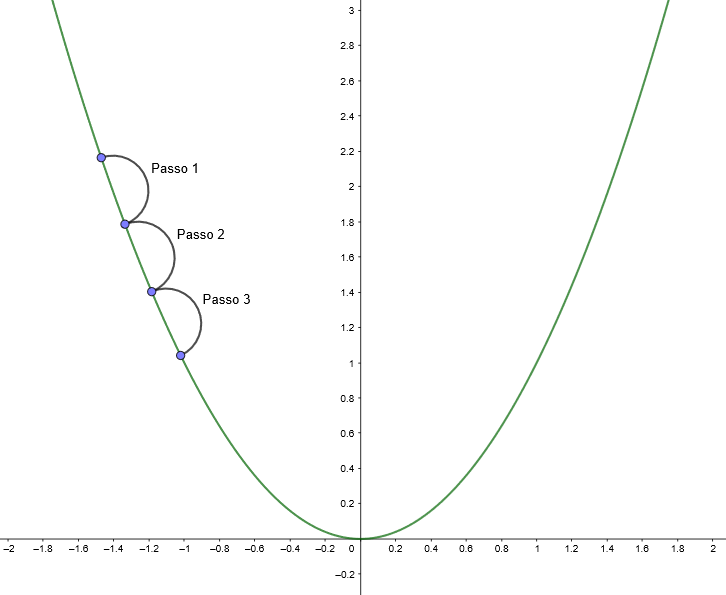
\includegraphics[height=7cm]{figuras/grad_1}
\caption{Visualização do método do gradiente descendente com taxa de aprendizado única. Os pontos azuis representam candidatos a ponto mínimo em cada iteração do algoritmo.}
\label{fig:grad_1}
\end{figure}

Podemos notar que as estimativas aproximam-se a uma velocidade constante do ponto de mínimo, que nesse caso ilustrativo é bem conhecido. Esse é o comportamento gerado por uma taxa de aprendizado fixa, e além disso com uma magnitude mediana. 

O que poderia acontecer se utilizarmos uma taxa de aprendizado muito grande é que com um passo do algoritmo, o ponto estimado poderia ir para o outro lado do arco da função, e depois retornar, e assim por diante, nunca convergindo para o mínimo, uma ilustração disso está na Figura \ref{fig:grad_2}.

\begin{figure}[htb]
\centering
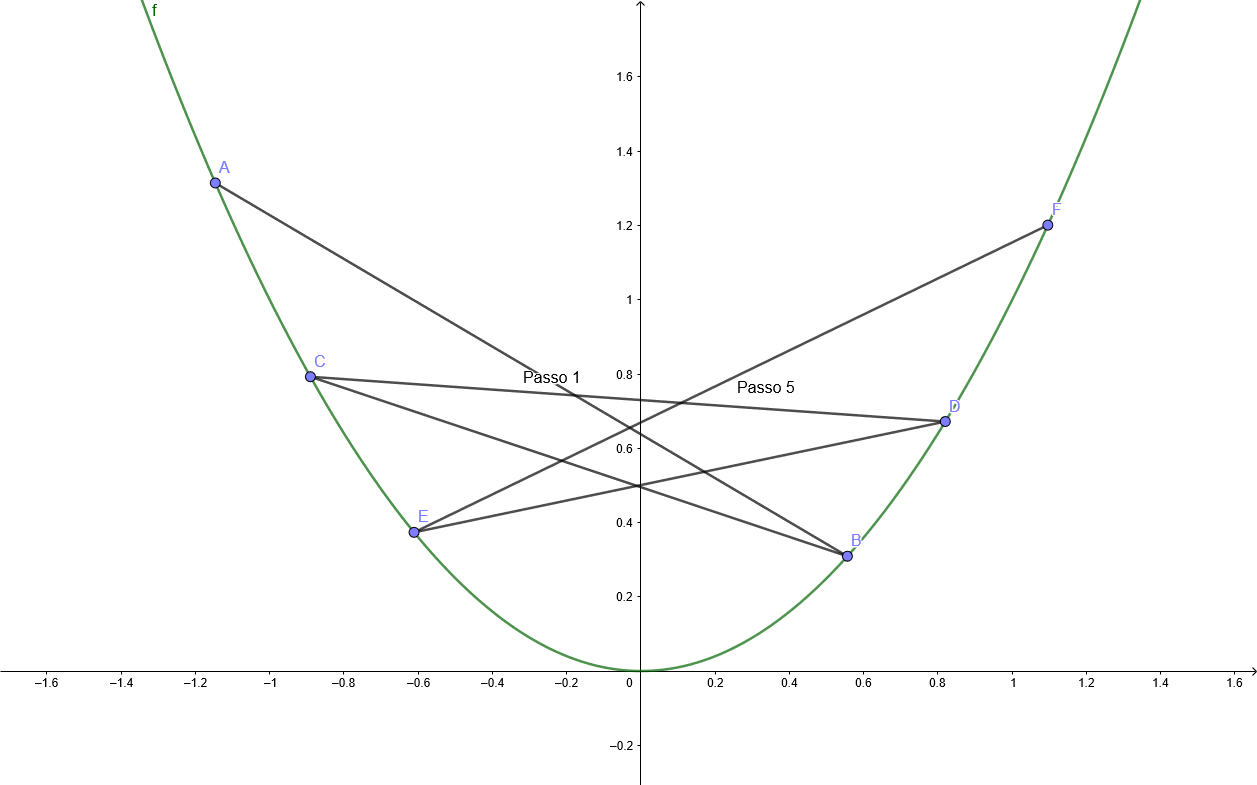
\includegraphics[height=7cm]{figuras/grad_2}
\caption{Visualização do método do gradiente descendente com taxa de aprendizado única. Ilustração do uso de um valor de taxa de aprendizado muito grande.}
\label{fig:grad_2}
\end{figure}

O caso oposto a este, ou seja, usar uma taxa muito pequena, claramente irá fazer com os passos dados sejam muito pequenos, e dessa forma o algoritmo demore muito a convergir, por isso é importante usar valores medianos que podem ser obtidos de forma heurística, embora na prática, conforme dito por Géron \citep{hands}, utiliza-se $\eta = 0.1$, sendo este um valor consensualmente utilizado pelo menos como ponto de partida.

A outra abordagem é utilizar valores variáveis, sendo o caso mais comum utilizar uma taxa que começa até mesmo maior do que o valor comum de $0.1$ mas que vai diminuindo a cada passo, numa tentativa de obter uma convergência mais rápida. Uma ilustração desse caso está na Figura \ref{fig:grad_3}.

\begin{figure}[htb]
\centering
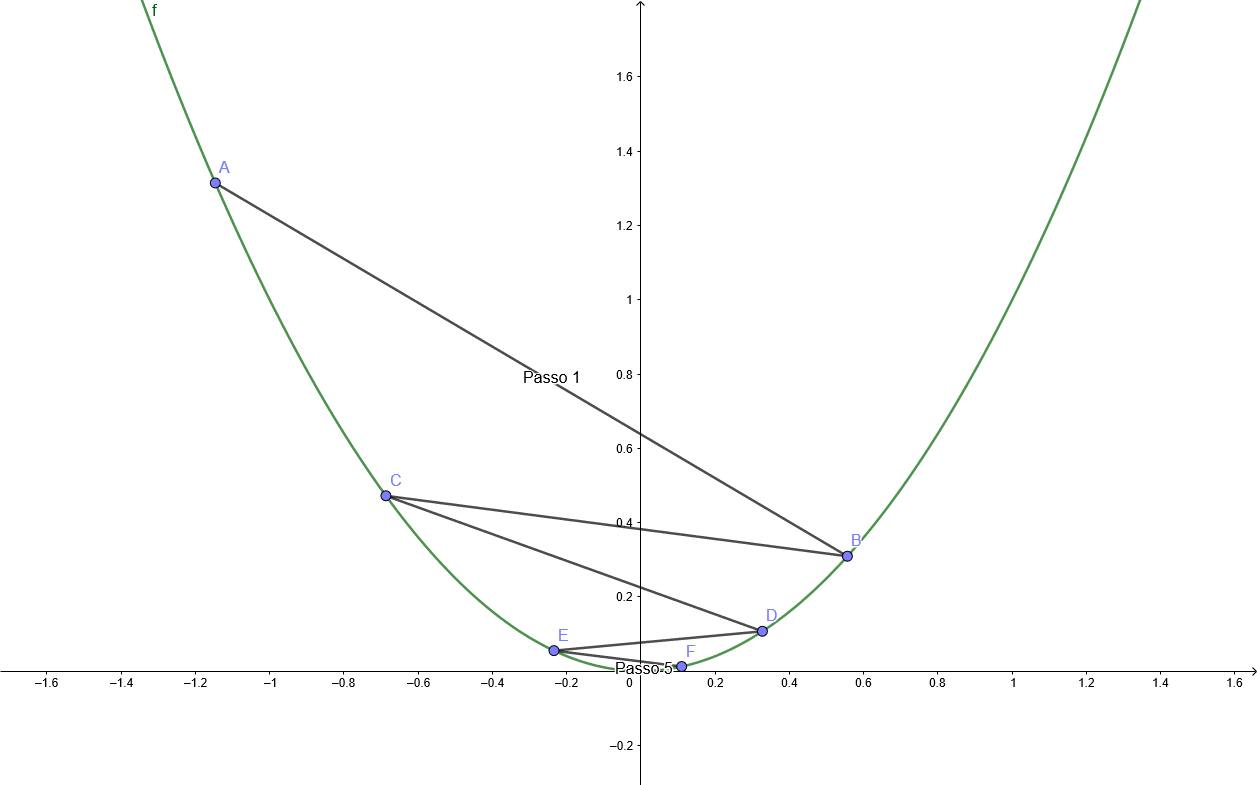
\includegraphics[height=7cm]{figuras/grad_3}
\caption{Visualização do método do gradiente descendente com taxa de aprendizado variável que vai diminuindo passo-a-passo do algoritmo.}
\label{fig:grad_3}
\end{figure}

Qualquer que seja o tipo de taxa de aprendizado que venha a ser utilizado, permanece como melhor estratégia testar qual deles irá gerar o melhor resultado, analisando diretamente os valores candidatos a mínimo obtidos pelo algoritmo como função do número do passo, criando assim outro tipo de gráfico, no qual não precisamos saber o formato da função objetivo, o que é razoável uma vez que não precisaríamos de um método numérico para obter seu ponto de mínimo.

Podemos observar este comportamento genérico para os 4 casos acima mencionados, na Figura \ref{fig:grad_4} temos os gráficos de valores hipotéticos de candidatos a mínimo gerados por (a) taxa de aprendizado fixa e grande, (b) taxa de aprendizado fixa e pequena, (c) taxa de aprendizado fixa e mediana, (d) taxa de aprendizado decrescente.

\begin{figure}[htb]
\centering
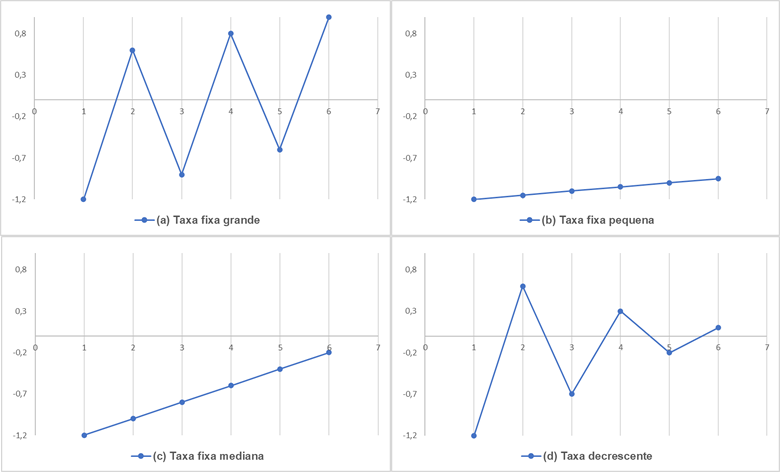
\includegraphics[width=14cm]{figuras/grad_4}
\caption{Comportamento de diferentes taxas de aprendizado nos valores candidatos a mínimo.}
\label{fig:grad_4}
\end{figure}

A partir deste comportamento geral, podemos testar nosso problema-alvo, verificar a qual comportamento ele mais se parece e assim decidir se devemos aumentar ou diminuir nossa taxa até obtermos um bom comportamento como aqueles vistos em (c) ou (d).


%%%%%%%%%%%%%%%%%%%%%%%%%%%%%%%%%%%%%%%%%%%%%%%%%%%%%%%%%%%%%%%%%%%%%%%%%%%%%%%%%%%%%%%%%%%%%%%

\chapter{Transformação de Box-Cox}
\label{ap:box-cox}

De forma a estabilizar a variância de séries temporais financeiras, faz-se necessária a aplicação de transformações não-lineares à série original, de forma a modelar a série transformada com os modelos $ARIMA$, que assumem uma variância constante, mesmo quando a média possui algumas tendências que podem ser compensadas aplicando-se diferenças, conforme visto no Capítulo \ref{cap:series}.

A transformação a seguir, criada por George Edward Pelham Box e David Roxbee Cox \citep{cox}, e conhecida por transformação de Box-Cox, é uma generalização da transformação logarítmica. Dada uma série temporal $Z_t$, a transformação é definida por:

\begin{equation}\label{eq:cox}
Z_t^{(\lambda)} = \left\{ \begin{array}{lr}\dfrac{Z_t^\lambda - 1}{\lambda},& \text{se } \lambda \neq 0\\\log{Z_t},& \text{se } \lambda = 0\end{array} \right.
\end{equation}

Onde, $\lambda$ é um parâmetro real que deve ser estimado. Para isso, Morettin e Toloi \citep{morettin} sugerem a análise de um gráfico que será construído a partir de dados da série temporal. No eixo das abcissas calculam-se médias de subconjuntos de observações, e no eixo das ordenadas, calculam-se as amplitudes de cada um desses subconjuntos.

Seja $Z_1, \ldots, Z_k$ um subconjunto de $k$ elementos da série temporal, definimos o par $(\bar{Z}, w)$ que será um ponto no gráfico, pelas componentes:

\[
\begin{array}{rl}
\bar{Z} =& \frac{1}{k}\sum_{i=1}^k Z_{t_i}\\
w =& \max(Z_{t_i}) - \min(Z_{t_i})
\end{array}
\]

Se, a partir desse gráfico, verificarmos que $w$ independer de $\bar{Z}$, ou seja, se os pontos estiverem espalhados ao redor de uma reta paralela ao eixo das abcissas, não haverá necessidade de transformação, pois assim a variância da série é estável, de acordo com Box e Jenkins \citep{box}. 

Se, por outro lado, $w$ for diretamente proporcional a $\bar{Z}$, ou seja, correlacionadas com uma reta com inclinação próxima de $45$ graus, então poderemos assumir que $\lambda = 0$. Por se tratar de um procedimento empírico, Box e Jenkins \citep{box} fornecem uma guia que pode ser utilizado para decidirmos por um valor adequado de $\lambda$. 

Exibido na Figura \ref{fig:box}, são dados possíveis gráficos que poderemos obter com esse procedimento e qual o valor correspondente de $\lambda$ que usaremos para aplicar a transformação \ref{eq:cox}.

\begin{figure}[htb]
\centering
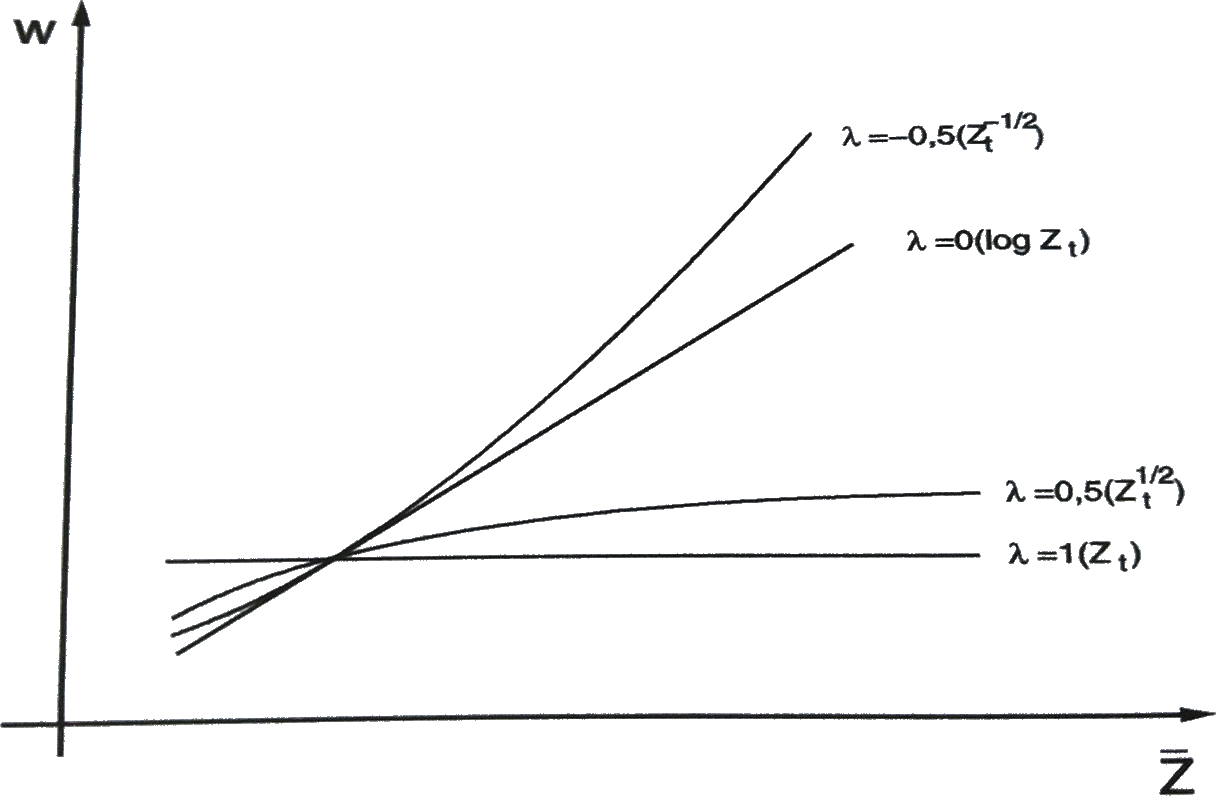
\includegraphics[width=8cm]{figuras/box}
\caption{Gráficos da amplitude por média de subconjuntos de $Z_t$, com os correspondentes valores de $\lambda$.\footnote{Extraido de Morettin e Toloi, 2019, pág 10.}}
\label{fig:box}
\end{figure} 



%%%%%%%%%%%%%%%%%%%%%%%%%%%%%%%%%%%%%%%%%%%%%%%%%%%%%%%%%%%%%%%%%%%%%%%%%%%%%%%%%%%%%%%%%%%%%%%

\chapter{Função de autocorrelação parcial}
\label{ap:facp}

A derivação da função de autocorrelação parcial mostrada abaixo, é extraída de Morettin e Toloi \citep{morettin}, nas páginas 138-140.

Suponha um modelo $AR(k)$ e seja $\phi_{kj}$ o seu $j$-ésimo coeficiente. Sabe-se que:

\[
\rho_j = \phi_{k1}\rho_{j-1} + \phi_{k2}\rho_{j-2} + \ldots + \phi_{kk}\rho_{j-k} \;,\;\;
j=1,\ldots,k
\]

A partir dessas $k$ expressões, obtemos as chamadas equações de Yule-Walker:

\begin{equation}\label{eq:yule}
\left[ \begin{array}{ccccc}
1 & \rho_1 & \rho_2 & \ldots & \rho_{k-1}\\
\rho_1 & 1 & \rho_1 & \ldots & \rho_{k-2}\\
 & \vdots &  & \ddots & \vdots\\
\rho_{k-1} & \rho_{k-2} & \rho_{k-3} & \ldots & 1
\end{array}  \right]
\left[ \begin{array}{c}
\phi_{k1}\\
\phi_{k2}\\
\vdots\\
\phi_{kk}
\end{array}  \right]
=
\left[ \begin{array}{c}
\rho_1\\
\rho_2\\
\vdots\\
\rho_k
\end{array}  \right]
\end{equation}

Resolvendo essas equações sucessivamente para $k=1, 2, \ldots$ obtemos:

\[
\begin{array}{rcl}
\phi_{11} & = & \rho_1 \\
\phi_{22} & = & \frac{\left| \begin{array}{cc}1&\rho_1\\\rho_1&\rho_2\end{array} \right|}{\left| \begin{array}{cc}1&\rho_1\\\rho_1&1\end{array} \right|}  \\
\phi_{33} & = & \frac{\left| \begin{array}{ccc}1&\rho_1&\rho_1\\\rho_1&1&\rho_2\\\rho_2&\rho_1&\rho_3\end{array} \right|}{\left| \begin{array}{ccc}1&\rho_1&\rho_2\\\rho_1&1&\rho_1\\\rho_2&\rho_1&1\end{array} \right|}\\
& \vdots &
\end{array}
\]

De modo geral, pode-se escrever:

\begin{equation}\label{defi:parcial}
\varphi_k := \phi_{kk} = \dfrac{|\mathbf{P}_k^{*}|}{|\mathbf{P}_k|}
\end{equation}

Onde nota-se que $\mathbf{P}_k$ é a matriz de autocorrelações do modelo $AR(k)$, e $\mathbf{P}_k^{*}$ é a matriz $\mathbf{P}_k$ com a última coluna substituída pelo vetor de autocorrelações, que é o termo à direita da igualdade das equações de Yule-Walker (\ref{eq:yule}).

Dessa forma, a definição acima de $\varphi_k$ é chamada de \emph{função de autocorrelação parcial} do \emph{lag} $k$, ou seja, de ordem autorregressiva $k$. Ela pode ser entendida como a correlação parcial entre as variáveis $Z_t$  e $Z_{t-k}$, ajustadas às variáveis intermediárias $Z_{t-1}, \ldots, Z_{t-k+1}$. Isto é, ela mede a correlação remanescente entre $Z_t$  e $Z_{t-k}$ depois de removida a influência de $Z_{t-1}, \ldots, Z_{t-k+1}$.